\documentclass[10pt, pdftex]{llncs}

\usepackage{graphicx}
\usepackage{color}
\usepackage{inputenc}
\usepackage{abbrevs}
\usepackage{paralist}
\usepackage{multirow}
\usepackage{subfigure}
\usepackage{listings}

\lstset{basicstyle=\ttfamily}
\lstdefinelanguage{cs}{
morekeywords={TOKENS,SYNTAXDEF,FOR,START,OPTIONS,TOKENSTYLES,RULES,COLOR,BOLD,DEFINE}
, morecomment=[l]{//}, morecomment=[s]{/*}{*/}, morestring=[b]", tabsize=2
}

\newcommand{\todo}[1]{\color{red}\textbf{TODO #1}\color{black}}

\def\lastname{Heidenreich, Johannes, Karol, Seifert, Wende}
  \title{Language Workbench Contest 2011\\EMFText, JaMoPP Solution}
  
  \author{Florian Heidenreich \and
  Jendrik Johannes \and
  Sven Karol \and\\
  Mirko Seifert \and
  Christian Wende}

  \institute{
    Institut f\"{u}r Software- und Multimediatechnik\\
    Technische Universit\"{a}t Dresden\\
    D-01062, Dresden, Germany\\
    \email{\{florian.heidenreich,jendrik.johannes,sven.karol,\\mirko.seifert,
c.wende\}@tu-dresden.de}
    }
    
\begin{document}

\maketitle

\begin{abstract}
This document contains a description of a solution to the Language
Workbench Competition 2011 built using the tools EMFText and JaMoPP. It may
serve as documentation for the EMFText tool and can be used in particular by users that
are new to EMFText or who want to compare this solution with the ones provided
by other language workbenches.
\end{abstract}

\section{Preliminaries}

To explore this solution in detail, you need to install the latest version of
EMFText from the EMFText update
site\footnote{\url{http://www.emftext.org/update}}. This document was created
at the time EMFText 1.3.1 was the latest release. Later releases may expose
different behavior. We'll try to keep this document up to date.

The source code of all the languages described in the following are available
from the EMFText Subversion
repository\footnote{\url{http://svn-st.inf.tu-dresden.de/svn/reuseware}}. The
languages start with the prefix \texttt{org.emftext.language.lwc11} and can be
found in folder \texttt{trunk/EMFText Languages/}.

\section{Phase 0 - Basics}

According to the task description of the Language Workbench Competition, this
section shows basic features of EMFText. This includes building a simple
structural DSL to define entities (Sect.~\ref{sec:phase-0-1}), defining
constraints on this language (Sect.~\ref{sec:phase-0-3}) and splitting models
into multiple files while cross-referencing elements in other files
(Sect.~\ref{sec:phase-0-4}). Generating code from DSL models is not supported by
EMFText. Nonetheless, we'll show how to use other EMF-based tools that are
especially suited for code generation in conjunction with the entity DSL
(Sect.~\ref{sec:phase-0-2}).

\subsection{Phase 0.1 Simple (structural) DSL}
\label{sec:phase-0-1}

To create new DSLs from the scratch, EMFText provides a wizard, which can be
invoked by selecting \texttt{File -> New -> EMFText project}. The wizard allows
to specify the following parameters to start the DSL development:

\begin{itemize}
  \item the name of the new metamodel
  \item the namespace prefix for the new metamodel
  \item the namespace URI for the new metamodel
  \item the name of the plug-in that will contain the metamodel
  \item the base package for the generated metamodel code
  \item the folder the metamodel (i.e., the \texttt{.ecore} and
        \texttt{.genmodel} file) and the syntax (i.e., the \texttt{.cs} file)
        will be stored in
  \item the name of the source folder to store the generated metamodel code in
  \item the file extension which shall be used for the files containing the
        textual DSL models
  \item the names of the Ecore file, the syntax definition file and the
        generator model
\end{itemize}

Usually it is sufficient to specify only a subset of these parameters and let
EMFText derive the others. If you need to make more custom settings, just
disable the \texttt{derive values from metamodel name} checkbox. In
Fig.~\ref{fig:newprojectwizard} the wizard completed with the settings we have
used for the Entity DSL is shown.

\begin{figure}
	\centering
	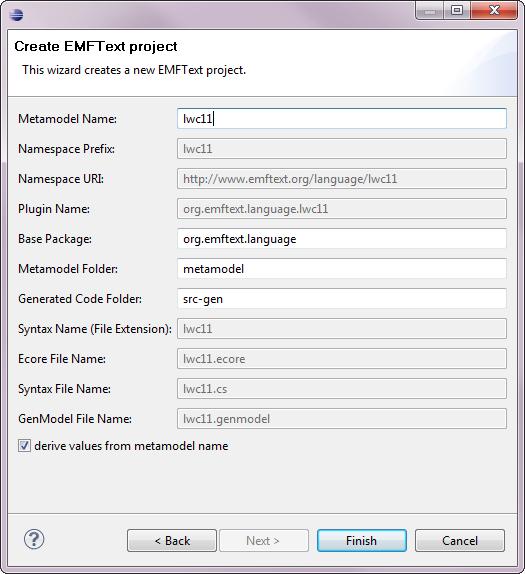
\includegraphics[width=0.60\textwidth]{figures/newprojectwizard.png}
	\caption{Creating a new project using the wizard}
	\label{fig:newprojectwizard}
\end{figure}

After pushing the \texttt{Finish} button, EMFText will create four plug-ins
yielding the workspace shown in Fig.~\ref{fig:newproject}. The workspace does
contain one plug-in that provides the parser runtime
(\texttt{org.emftext.commons.antlr3\_2\_0}), one plug-in that hosts the
metamodel (\texttt{org.emftext.language.lwc11}) and two plug-ins the implement
the DSL functionality (\texttt{...lwc11.resource.lwc11} and
\texttt{...lwc11.resource.lwc11.ui}).

\begin{figure}
	\centering
	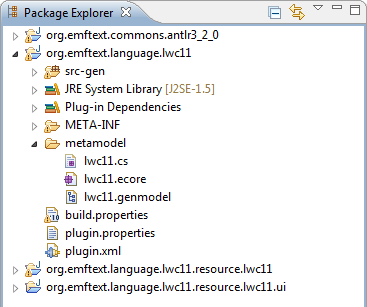
\includegraphics[width=0.60\textwidth]{figures/newproject.png}
	\caption{Workspace after creating the new project}
	\label{fig:newproject}
\end{figure}

EMFText does require an existing metamodel before one can start defining the
textual syntax for the language. Therefore, we need to create an \texttt{.ecore}
model for the DSL. We used the sample tree editor provided by EMF, but other
editors (e.g., the TextEcore DSL
editor\footnote{\url{http://www.emftext.org/language/textecore}}) can be used
as well.

We decided to split the metamodel into two files (i.e., \texttt{lwc11.ecore} and
\texttt{types.ecore}) to allow the creation of type libraries independent of
the entity models. The definition of these two metamodels is
straighforward\footnote{The types created by the new project wizard need to be
removed from \texttt{lwc11.ecore}}. To model types, we define an abstract
metaclass \texttt{NamedElement}, a metaclass \texttt{Type}, which subclasses 
\texttt{NamedElement} and a further subclass \texttt{PrimitiveType}. Also, a 
metaclass \texttt{TypeLib} models a container
for a set of types. To model entities, we use the metaclass
\texttt{Entity}, which inherits from \texttt{Type} as entities are supposed to
function as types. Each \texttt{Entity} holds a set of features, whereas an
\texttt{EnitityModel} can be used to group multiple \texttt{Entity} elements.
The resulting metamodels are shown in Fig.~\ref{fig:metamodel1}.

\begin{figure}
	\centering
	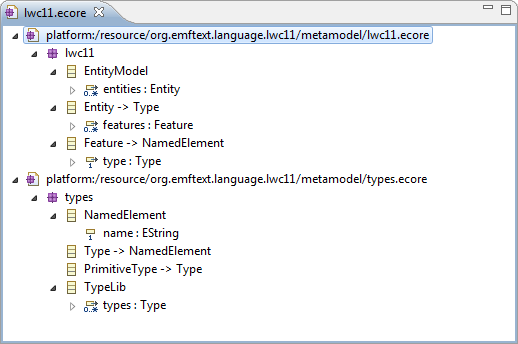
\includegraphics[width=1.00\textwidth]{figures/metamodel1.png}
	\caption{Initial metamodel of the Entity DSL}
	\label{fig:metamodel1}
\end{figure}

After designing the metamodel for types and entities, the actual syntax
development with EMFText can start. The new project wizard did already create a
sample \texttt{.cs} file, which needs to be adjusted to our new metamodels. To
define syntax for entities, three basic syntax rules are sufficient. These are
shown in Listing~\ref{lst:simplesyntax}.

\lstinputlisting[label=lst:simplesyntax,caption=Initial syntax for the Entity
DSL,language=cs]{listings/simplesyntax.cs}

An EMFText syntax specification starts with a declaration of the file extension
which will be used for the DSL models (line 1). This is followed by a reference
to the metamodel we'd like to define syntax for (line 2). We do not need to
explicitly tell EMFText where to find this metamodel, because the name of the
\texttt{.genmodel} file is equal to the name of the syntax specification. Note
that EMFText references the generator model instead of the \texttt{.ecore}
model, because it requires information about the generated metamodel code, which
is only available in the former model. In line 3 the start symbol is set to be
\texttt{EntityModel}. Objects of this class will form the root of the Entity DSL
models.

Then, syntax is defined for the three metaclasses \texttt{EntityModel},
\texttt{Entity} and \texttt{Feature} (lines 6 to 8). The syntax for objects of
type \texttt{EntityModel} starts with an optional list of imports---each
represented by the keyword \texttt{import} and a URI enclosed in angle brackets.
These are not required yet, but we'll need them in Sect.~\ref{sec:phase-0-4}.

Then, text for the contained entities (\texttt{entities*}) can follow. Entities
theirself are represented by the keyword \texttt{entity}, followed by their name
and the set of contained features enclosed in curly brackets. The syntax for the
name attribute is defined as \texttt{name[]}, which states that names must
adhere to the predefined token \texttt{TEXT}, which is similar to Java identifiers
(i.e., it must not contain spaces). Finally, the syntax for features is defined
to consist of the type and the name of the feature. Again, the \texttt{TEXT}
token is implicitly used here. As \texttt{type} is a non-containment reference,
we can see that both EAttributes (e.g., \texttt{name}) and non-containment
EReferences must specify the token which can be used to represent them. Containment reference do not require this,
since they are represented by a syntax rule (i.e., the rule for the type of the
reference) rather than a single token.

\begin{figure}
	\centering
	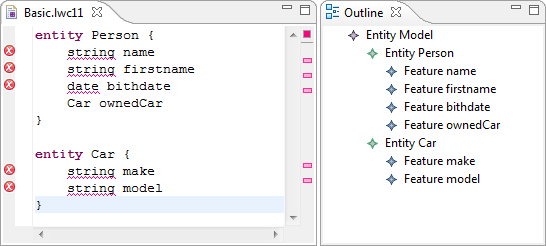
\includegraphics[width=1.00\textwidth]{figures/examplefile1.png}
	\caption{Example entity model (types not resolving yet)}
	\label{fig:example1}
\end{figure}

After generating the DSL tooling from this \texttt{.cs} specification by
invoking a right-click on the \texttt{lwc11.cs} file and selecting
\texttt{Generate Text Resource}, we're ready to create textual entity models.
Figure~\ref{fig:example1} shows an example model. You can create such models by
firing up a second Eclipse instance and creating a new \texttt{lwc11} file using
\texttt{File -> New -> EMFText .lwc11 file}.

One can see that the primitive types used in Fig.~\ref{fig:example1} (e.g.,
\texttt{string} and \texttt{date}) cannot be resolved yet. The complex types
(i.e., other entities) can be resolved using the default reference resolving
which is generated by EMFText. For example, the type of reference
\texttt{Person.ownedCar} is correctly resolved to refer to the entity
\texttt{Car} which is also defined in the example file.

To resolve primitive types correctly, we can create a library for primitive
types. We did so by performing a right-click on EClass \texttt{TypeLib}
and selecting \texttt{Create Dynamic Instance} in the sample Ecore tree editor.
We created a simple library containing three primitive types (\texttt{string},
\texttt{date} and \texttt{int}) and stored it in
\texttt{modellib/primitivetypes.xmi}. One can also define textual syntax for
primitive types, but we choose to use the XMI representation to show that
DSLs generated by EMFText do smoothly integrate with other EMF-based resources.

Now, to resolve references to primitive types correctly, we need to load the
created library (i.e., \texttt{primitivetypes.xmi}) and look up types by their
name, whenever resolving types is requested. To ease this task, EMFText has
generated a class \texttt{FeatureTypeReferenceResolver} which resides in the
\texttt{src} folder of the \texttt{...lwc11.resource.lwc11} plug-in. The
generated implementation of this class delegates all calls to a default
reference resolver.

We need to change the method \texttt{resolve()} which is called whenever a
non-containment reference needs to be resolved. To find the primitive types, we
load the \texttt{primitivetypes.xmi} resource, search for a type with the
correct name and add a mapping for this type if the name matches the identifier
that must be resolved. For details on this implementation you may want to have a
closer look at the \texttt{FeatureTypeReferenceResolver} class.

After implementing this resolution algorithm which is about 20 lines of Java
code, the primitive types can be found and the editor shows the same Entity DSL
model without any errors (see Fig.~\ref{fig:example2}).

\begin{figure}
	\centering
	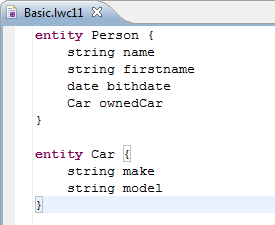
\includegraphics[width=0.50\textwidth]{figures/examplefile2.png}
	\caption{Example entity model (types resolved now)}
	\label{fig:example2}
\end{figure}

EMFText itself does not provide dedicated support to customize reference
resolving. You can either stick with the default resolving mechanism, which is 
already quite smart, or implement your own resolution strategy in Java. To use
more sophisticated techniques for reference resolution you may want to consider
using JastEMF\footnote{\url{http://code.google.com/p/jastemf}} or EMF Attribute
Grammars\footnote{\url{http://emftext.org/index.php/EMFText\_Concrete\_Syntax\_Zoo\_EAG}}.

\subsection{Phase 0.2 Code generation to GPL}
\label{sec:phase-0-2}

To obtain code for a General Purpose Language such a Java or C\# for the
Entity DSL models, there is two possibilites. First, you can use a Model-2-Text tool of
your choice (e.g.,
JET\footnote{\url{http://www.eclipse.org/emft/projects/jet}},
Acceleo\footnote{\url{http://www.eclipse.org/acceleo}} or
Xpand\footnote{\url{http://www.eclipse.org/modeling/m2t/?project=xpand}}).
EMFText itself is specifically built to map between models and text that
represent \emph{the same} language. If you want to transform the Entity models
to another language you're better of using one of the tools listed above. In
particular the tools that are based on EMF should be able to load Entity models
without any problems. There is no need to transform the textual models to XMI as
EMF takes care of using the correct plug-in to load the models from their
textual representation.

Second, if you're lucky and there is a metamodel and a textual syntax of your
GPL available, you can use a Model-2-Model transformation instead of a
Model-2-Text tool. For the Java language, a metamodel and syntax is available
from the JaMoPP homepage\footnote{\url{http://www.jamopp.org}}. Thus, you can
use an arbitrary M2M tool (e.g., ATL or
QVTO\footnote{http://www.eclipse.org/m2m/}). The advantage of this procedure is
that your transformation will produce a correctly structured model of a Java
programm instead of plain text.

As code generation is not an objective of EMFText, we did not perform this task
for the Entity DSL, but you can find an example on how to generate Java code
from UML models with ATL on the JaMoPP
homepage\footnote{\url{http://www.jamopp.org/index.php/JaMoPP\_Applications\_ATL}}.

\subsection{Phase 0.3 Simple constraint checks}
\label{sec:phase-0-3}

Performing constraint checks on the Entity DSL models can be achieved in
different ways. First, EMFText integrates with the EMF Validation Framework.
Thus, any registered validator for your metamodel will be called by the
generated editor and errors will be shown. You can also use dedicated constraint
languages (e.g., OCL or EVL\footnote{\url{http://www.eclipse.org/gmt/epsilon/doc/evl}}).

Second, EMFText allows to register post processors, which are called after
models are created from text. Such post processors can be used to check constraints
using Java code. Simply put, you can register a class with one of the
extension points that is defined by the \texttt{...lwc11.resource.lwc11}
plug-in, add some code which inspects your models and attaches errors to it if
constraints are violated. You can consult the EMFText User
Guide\footnote{\url{http://www.emftext.org/index.php/EMFText\_Documentation}} 
for more detailed information on how to implement such a post processor.

\lstinputlisting[label=lst:postprocessor,caption=Post processor that detects
duplicate names,language=Java,tabsize=2]{listings/ConstraintChecker.java}

To show at least a basic example, consider Listing~\ref{lst:postprocessor} which
show a post processor class that check that there are no duplicate names. Once
this post processor is correctly registered using the Eclipse extension
mechanism, duplicate name will we marked in the editor. The result is shown in
Fig.~\ref{fig:duplicatenames}.

\begin{figure}
	\centering
	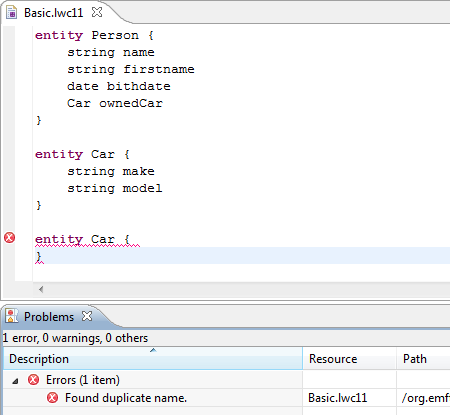
\includegraphics[width=0.70\textwidth]{figures/duplicatename.png}
	\caption{Duplicate name detection}
	\label{fig:duplicatenames}
\end{figure}

It is good practice to put the constraint checking classes into separate
plug-ins. For example, the class \texttt{ConstraintChecker} from 
Listing~\ref{lst:postprocessor} can be found
in the \texttt{org.emftext.language.lwc11.constraints} plug-in. In contrast to 
registering validation classes with the Eclipse Validation Framework, the post
processors are only called by EMFText editors and not by other editors for the
same metamodel. If you have multiple concrete syntaxes (e.g., a textual and a
graphical one) it is better to implement constraint checks based on the Eclipse
Validation Framework.

\subsection{Phase 0.4 Splitting models}
\label{sec:phase-0-4}

\begin{figure}
	\centering
	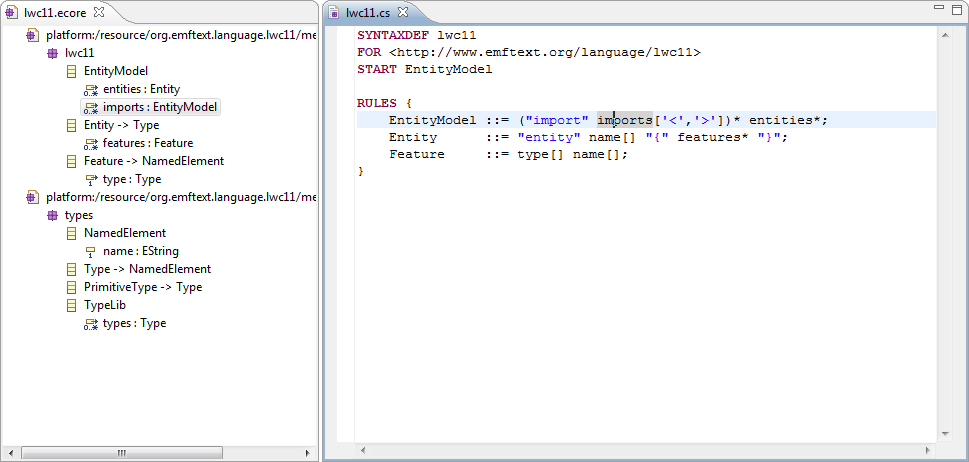
\includegraphics[width=1.00\textwidth]{figures/imports.png}
	\caption{Metamodel extension and syntax for imports}
	\label{fig:imports}
\end{figure}

\begin{figure}
	\centering
	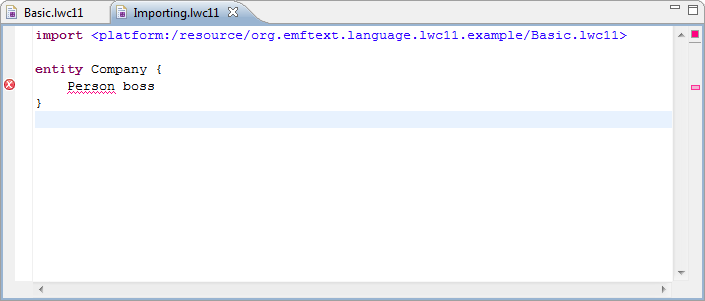
\includegraphics[width=1.00\textwidth]{figures/importexample1.png}
	\caption{Example entity model with import (Resolving not working yet)}
	\label{fig:importexample1}
\end{figure}

\begin{figure}
	\centering
	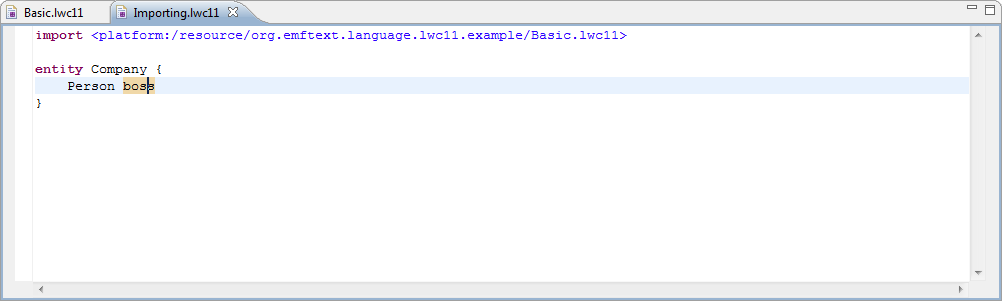
\includegraphics[width=1.00\textwidth]{figures/importexample2.png}
	\caption{Example entity model with import (Resolving now working)}
	\label{fig:importexample2}
\end{figure}


\section{Phase 1 - Advanced}

\subsection{Phase 1.1 Language integration}

\subsection{Phase 1.2 Implementing runtime type systems}

\subsection{Phase 1.3 Model-to-model transformation}

\subsection{Phase 1.4 Visibilities, namespacess and scoping for references}

\subsection{Phase 1.5 Integrating manually written code}

\subsection{Phase 1.6 Multiple generators}

\section{Phase 2 - Non-Functional}

\subsection{Phase 2.1 Evolving the DSL without breaking existing models}

\subsection{Phase 2.2 Working with models in a team}

\subsection{Phase 2.3 Scalability of the tools}

\section{Phase 3 - Freestyle}

\begin{itemize}
  \item Use EMFDoc and show documentation in generated editor
\end{itemize}

\section*{Acknowledgement}
\small
	\todo{Update.}
    This research has been co-funded by the European Commission within the 6th Framework Programme project
    \textsc{Modelplex} \#034081, the 7th Framework programme project
    \textsc{MOST} \#216691 and by the German Ministry of Education and Research
    within the project feasiPLe.

\bibliographystyle{splncs}
%\huge
\bibliography{biblio}

\end{document}
